%%%%%%%%%%%%%%%%%%%%%%%%%%%%%%%%%%%%%%%%%%
% Master Thesis 
% Polina Polunina
% October 2022 
%
% License:
% CC-BY-SA 4.0 -- Creative Commons Attribution-ShareAlike 4.0 International
% https://creativecommons.org/licenses/by-sa/4.0/legalcode
%%%%%%%%%%%%%%%%%%%%%%%%%%%%%%%%%%%%%%%%%%
\section{State-of-the-art}

From the beginning of the COVID-19 pandemic, several approaches have been presented to determine SARS-CoV-2 in wastewater samples. An overview of existing tools and pipelines will be given in \cref{sec:prior:methods}. Some tools and pipelines aiming to detect SARS-CoV-2 lineages and their abundance in wastewater samples will be considered. More specifically, \cref{sec:prior:methods:tools} will show individual tools that require data preprocessing and/or need to be plugged into pipelines before they can be used, while \cref{sec:prior:methods:pipelines} will demonstrate standalone pipelines that do all the analysis from raw data to determining lineages and their abundances. This determination can be focused on \acrfull{vocs} as well as \acrfull{vois} and additionally with an intention to detect newly appeared unknown variants. In \cref{sec:prior:discussion}, a short discussion of the existing methods with respect to the goals of this thesis will be given.

    \subsection{Methods for wastewater surveillance} \label{sec:prior:methods}
    
        \subsubsection{Individual tools} \label{sec:prior:methods:tools}

        \paragraph{Freyja}
        One optimized approach for virus concentration from wastewater is proposed by Karthikeyan et al. \cite{karthikeyan2022}, they developed developed a tool called Freyja that detects variants from SARS-CoV-2 RNA sequencing and estimates the relative abundance of SARS-CoV-2 lineages. To represent each SARS-CoV-2 lineage in the global phylogeny, Freyja uses a barcode library of lineage-defining mutations \cite{wastewater2022,mcbroome2021}. These lineage-determining mutational barcodes derived from the UShER \cite{usher} global phylogenetic tree as a basis set to solve the constrained (unit sum, non-negative) de-mixing problem. For each lineage-defining mutation, Freyja stores the \acrfull{snv} frequencies (the proportion of reads that contain the \acrshort{snv}) for each sample. In order to recover relative lineage abundance, Freyja solves a depth-weighted least absolute deviation regression problem, a mixed sample analog to minimize edit distances between sequences and a reference, based on \acrshort{snv} frequencies at positions with greater sequencing depth. In order to guarantee meaningful results, Freyja constrains the solution space such that each lineage abundance value is non-negative and the overall lineage abundance sums to one. Site-specific weighting is applied by Freyja to account for non-constant variance in measured \acrshort{snv} frequency across sites, which enables prioritizing information according to sequencing depth at each site. Because of using log-transformed read depths, the data is robust to common characteristics of real sequencing data, such as heavily skewed depths across amplicons \cite{karthikeyan2022}.

        As Freyja uses UShER phylogenetic tree, it is a good solution for users, for example, politicians or journalists, that chase only high-level information to know which variants are relevant and the most ubiquitous at this time point. The information about the proportion of specific SARS-CoV-2 lineages (e.g. Alpha, Delta, Omicron, etc.) and their co-occurrences in certain areas could be useful for some rough reports that are needed for political or mass media goals. Since using UShER bar codes, we know the names of lineages without details, that could be a good solution. 
        \paragraph{COJAC}
        In parallel, based on SARS-CoV-2 RNA amplicon sequencing for wastewater samples in two cities in Switzerland, Jahn and co-authors used a bioinformatics method called Co-Occurrence Adapted Analysis and Calling (COJAC) \cite{jahn2022} to detect the local spread of Alpha, Beta and Gamma variants in the virus. For detection, COJAC searches for read pairs with multiple variant-specific mutations. 
        
        The COJAC \cite{jahn2021,jahn2022} package comprises a set of command-line tools to analyze the co-occurrence of mutations on amplicons. It is useful, for example, for the early detection of viral variants of concern in environmental samples, and has been specifically designed to scan for multiple SARS-CoV-2 variants in wastewater samples \cite{cojac2022}.
        
        Similarly to Freyja, COJAC is able to detect outbreaks more than two weeks before the first positive clinical tests were reported. Compared to the Freyja tool, COJAC results can be used for downstream analysis that afterward can be imported to CoV-spectrum \cite{chen2022b}, an interactive platform aiming to assist scientists in investigating and identifying SARS-CoV-2 variants, and it can be interesting for researchers and scientists that need more details about not only the names of SARS-CoV-2 lineages, that are listed in UShER phylogenetic tree but also new variants that are yet unknown. The usage of CoV-Spectrum tool for downstream analysis is supposed to be up-to-date and to show dynamics. This can be used to give information about new variants and new patterns that can be described as suspicious.
        \paragraph{LCS}
        Another tool that estimates the relative frequencies of SARS-CoV-2 variants in pooled samples, LCS \cite{valieris2022}, uses a statistical model. The model takes into account previously defined genomic polymorphisms that characterize SARS-CoV-2 variants. The tool supports both raw sequencing reads for polymorphism-based markers calling and predefined markers in the \acrlong{vcf}. Similarly to Freyja, LCS tool uses Pango designation, and it is able to use UShER bar codes which is not the case for COJAC.
        \paragraph{Kallisto}
        Among other methods, Kallisto \cite{bray2016} was initially developed for quantifying abundances of transcripts from RNA-Seq data, or, more generally, of target sequences using high-throughput sequencing reads. It is based on the idea of pseudoalignment for rapidly determining the compatibility of reads with targets, without the need for alignment. 
        
        In spite of tools listed above, Freyja, COJAC, and LCS, Kallisto initially was not developed with focus on SARS-CoV-2. Recently, Kallisto tool was repurposed to analyze SARS-CoV-2 in wastewater samples \cite{baaijens2021,kallisto2022}. Due to the genome's division into regions that code different proteins, it was thought that it should only be sequenced in the region that codes the spike protein, which is used by the virus to attach to its hosts. Sites on the spike and nucleocapsid proteins are mainly affected by adaptive evolution in SARS-CoV-2 \cite{rochman2021}. As a viral nucleocapsid protein, it binds to the genomic RNA sequence and enters the host cell. As long as Kallisto is used on those regions, the algorithm is able to distinguish virus variants. Both \cite{baaijens2021} and \cite{anton2022} provide confirmation of this since the region coding for spike protein seems to fit better in the algorithm than sequencing the whole genome. However, Kallisto has limited capability to detect clinical variants with a frequency of <10\%, and background noise was observed to be 0.01-0.09\% \cite{baaijens2021}.
        \paragraph{Alcov}
        A tool called Alcov \cite{ellmen2021} is another option for learning the abundance of SARS-CoV-2 variants. For each mutation, Alcov calculates its frequency as the number of single-nucleotide variants divided by the number of reads covering that base. The Alcov algorithm only considers locations with at least 40 reads of coverage in order to reduce the variance of the estimates. Whenever a mutation contains multiple nucleotide polymorphisms, Alcov assigns its prevalence to the nucleotide polymorphism with the highest frequency. \acrfull{ols}, a well-studied problem in statistics that can be solved efficiently, are used to calculate relative abundance for each \acrfull{voc} lineage. As COJAC, Alcov works with amplicons. When comparing Alcov method with COJAC approach, Alcov considers reads carrying mutations when estimating lineages cooccurrences, while COJAC considers amplicons carrying mutations.
        \paragraph{SAM Refiner}
        A further method called SAM Refiner is a part of the workflow developed by Devon A. Gregory et al. \cite{gregory2021} based on amplicon sequencing of SARS-CoV-2 spike domains in order to track viral populations in wastewater. In June 2021, Devon A. Gregory and colleagues were able to detect the appearance of two variants of concern, Alpha and Gamma, and their displacement of the D614G B.1 variant in a Missouri sewer shed with the help of SAM Refiner. This tool can report novel variants and remove chimeric sequences generated by \acrshort{pcr}. Comparing SAM Refiner with above listed methods, SAM Refiner has a feature of removing errors associated with PCR, such as single-nucleotide polymorphisms (SNPs) and chimeric sequences which is not suggested by Freyja, COJAC, Kallisto, and Alcov tool. Moreover, by using this tool, variant reports are generated that include SNPs, multiple nucleotide polymorphisms (MNPs), insertions, deletions, and downstream amino acid changes, as well as PCR-created chimeric sequences are removed. 
        
        \subsubsection{Standalone pipelines} \label{sec:prior:methods:pipelines}
        \paragraph{Pipeline proposed by Pipes et al.}
        In the method proposed by Pipes et al. \cite{pipes2022}, unlikely lineages are initially removed, missing nucleotides are imputed using the global SARS-CoV-2 phylogeny, and the proportion of lineages is estimated using an Expectation-Maximization algorithm \cite{dempster1977}. There are two components of the method: estimating proportions of SARS-CoV-2 lineages and imputation of SARS-CoV-2 reference lineages. The imputation component is a specificity of the method proposed by Pipes et al., compared to other methods described above, like Freyja, COJAC, SAM Refiner, etc. This component's purpose is to reduce a problem when estimating the fraction of different SARS-CoV-2 strains. A problem can arise because a large number of SARS-CoV-2 sequences submitted to public databases contain missing data (i.e., bases that are not coded as A, G, C, or T). Thus, when compared to sequencing reads, strains with a high proportion of missing data will contain fewer nucleotide differences. While using an imputation approach, it is possible to allow for a like-to-like comparison of reads against all reference strains. The method was initially applied to wastewater samples collected across the San Francisco Bay Area and showed promising results.
        \paragraph{Gromstole}
        Yet another concept for estimating the relative frequencies of different SARS-CoV-2 lineages in wastewater samples is pipeline Gromstole \cite{gromstole2022}. Gromstole provides a set of scripts, including a Python script for rapidly extracting coverage and mutation frequency statistics from the reference mapping program minimap \cite{li2018}, and an R script that estimates the frequency of a variant of concern from the frequencies of mutations associated with the constellation file, using quasibinomial regression. The other R script is used to visualize variant frequency estimates across a set of samples.
        \paragraph{AG}
        Another approach, AG pipeline, is a suite of tools \cite{nguessan2022}. A pipeline was successfully applied to 936 wastewater samples and thousands of matched clinical sequences collected in Montreal, Quebec City, and Laval between March 2020 and July 2021. To calculate SARS-CoV-2 lineage frequencies within a sample, a linear model was fitted to the signature mutations data to calculate within-sample frequency. This approach is based on the assumption that the frequency of mutations within a sample is a linear combination of the frequency of the lineages and the prevalence of mutations within their consensus sequences. 
        \paragraph{Lineagespot}
        Pechlivanis et al., in turn, proposed a framework, called Lineagespot \cite{pechlivanis2022}, for monitoring mutations and detecting SARS-CoV-2 lineages in wastewater samples. Using next-generation sequencing data from 14 wastewater samples covered by a 6-month period collected from the municipality of Thessaloniki, Greece, the method was tested and evaluated. 

        With Trim Galore \cite{krueger2021}, Lineagespot performs quality control and adapter trimming on raw \acrshort{fastq} files. To map reads to reference SARS-CoV-2 sequences, minimap2 \cite{li2018} is used. Primer trimming is performed using SAMtools \cite{li2009}, BEDTools \cite{bedtools}, and minimap2. By using Picard \cite{picard}, duplicates obtained from the sequencing process can be filtered. Then, Lineagespot uses FreeBayes \cite{garrison2012} to call variants and SnpEff \cite{snpeff} to annotate mutations. Then, for the lineage assignment process, in order to retrieve lineage definitions, Lineagespot relies on particular sources. For Lineagespot, two sources can be used: lineage-characteristic mutation profiles derived from (i) outbreak.info \cite{outbreakinfo}, and (ii) trained Pangolin \cite{otoole2021} models. As a result of the pipeline, a tabular output contains the most probable lineages found. The diagram that describes the lineagespot workflow is presented in \cref{fig:prior:ls}.
        
        After computing lineages abundances, Lineagespot provides a set of indicators for each of the provided references. Based on these indicators, the final assignment is made. This additional step in Lineagespot is one of the advantages of this pipeline over others since it allows to mitigate the risk of wrong assigned lineages (e.g. in the case of two groups of reads satisfying different rules for the same lineage but reads from both groups never satisfying all rules for this lineage). According to Lineagespot, several different indicators reflect how many rules are satisfied, how many rules are satisfied based on the detected mutations, and how many reads support each rule both as a reference and as an allele. The drawback of this method is that assignment is made by a semi-automated process but not completely automated.
        \begin{landscape}
        \centering\vspace*{\fill}
        \begin{center}
        \begin{figure}[H]
        	\centering
            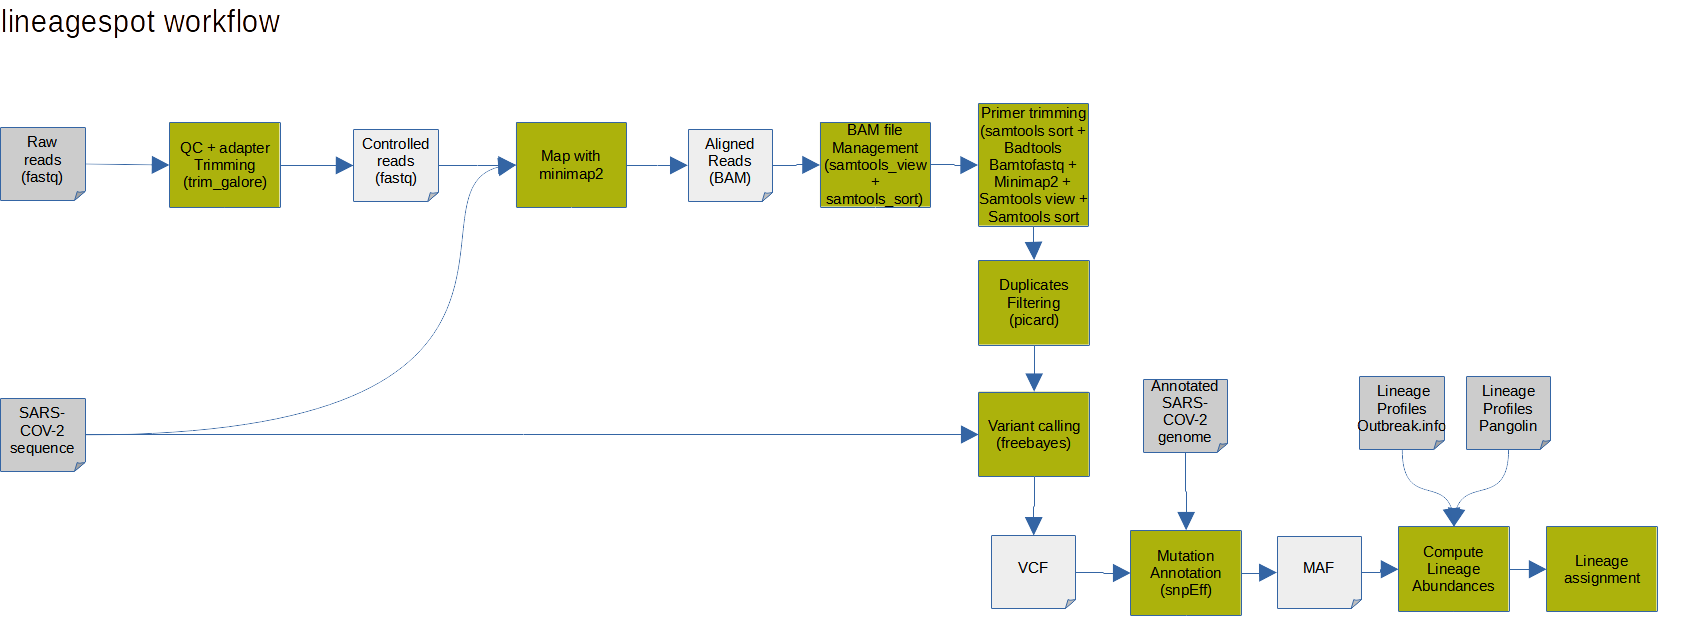
\includegraphics[width=1.4\textwidth]{figures/prior/lineagespot.png}
            \captionof{figure}{Lineagespot workflow.}
            \label{fig:prior:ls}
        \end{figure}
        \end{center}
        \vfill
        \end{landscape}
        
        \paragraph{PiGx}
        The other pipeline, PiGx SARS-CoV-2 \cite{schumann2021}, first, performs extensive quality control on the raw reads and information about primers and adapters used. Fastp \cite{chen2018} is used for adapter trimming and filtering, while iVAR is used for primer trimming. Using BWA \cite{li2013}, the trimmed reads are aligned to the reference genome of SARS-CoV-2, resulting in SAM/BAM files with aligned and unaligned reads. After alignment, MultiQC \cite{multiqc} is used to aggregate reports that check the quality of raw and processed reads. Further, PiGx checks samples for genome coverage and how many of the provided signature mutation sites, sites with mutations that characterize variants of concern or variants of interest, are covered by the sample. Every sample is given a quality score based on this. Those samples with genome coverage of less than 90\% are discarded from time series analyses and summaries.

        With LoFreq \cite{lofreq}, variants are called, and \acrshort{snvs} are inferred from aligned reads. The mutations are annotated with \acrshort{vep} \cite{mclaren2016}. 
        
        PiGx is capable of deconvoluting the frequencies of variants of concern from pooled sequencing reads. Briefly, the deconvolution method uses signature mutations for each variant of concern and tries to discern the proportions of these variants making up the observed mutation frequencies in the pooled sequencing reads obtained from the wastewater. To infer the proportions of each lineage on each sample, the deconvolution method is applied (based on the frequencies of the signature mutations). On the basis of the observed frequencies of signature mutations for each lineage, the lineage frequencies are predicted using a regression model. 
        
        After lineage frequencies prediction, PiGx generates a per-sample report that describes variants of concern and frequency of lineages from each wastewater sample. Additionally, the unaligned reads will be taxonomically classified with Kraken2 \cite{wood2014,wood2019,lu2020} to determine the abundance of RNA that matches other existing species found in unaligned reads in the wastewater samples. The diagram of PiGx pipeline is shown in \cref{fig:prior:pigx}.
        
        One of the significant benefits of PiGx method is the addition of different weights of tracked lineages based on how many signature mutations were found for each of them for a given sample. The purpose of this step is to determine which lineages have a low abundance and have only a few or only shared mutations in order to obtain more precise predictions. 

        PiGx has another advantage - controlling taxonomic classification for other species present in samples but not mapped to the SARS-CoV-2 reference sequence. With Kraken2 usage, this simple step opens opportunities for learning about sample diversity. Due to Kraken2's k-mer classification, it can also identify reads that match SARS-CoV-2 but are not aligned with stringent alignment tools. In addition, it provides insights into the possibility of losing new mutations that weren't captured in the alignment. The user can analyze potential issues here and adjust the alignment stringency if necessary.
        \begin{landscape}
        \centering\vspace*{\fill}
        \begin{figure}[H]
        	\centering
            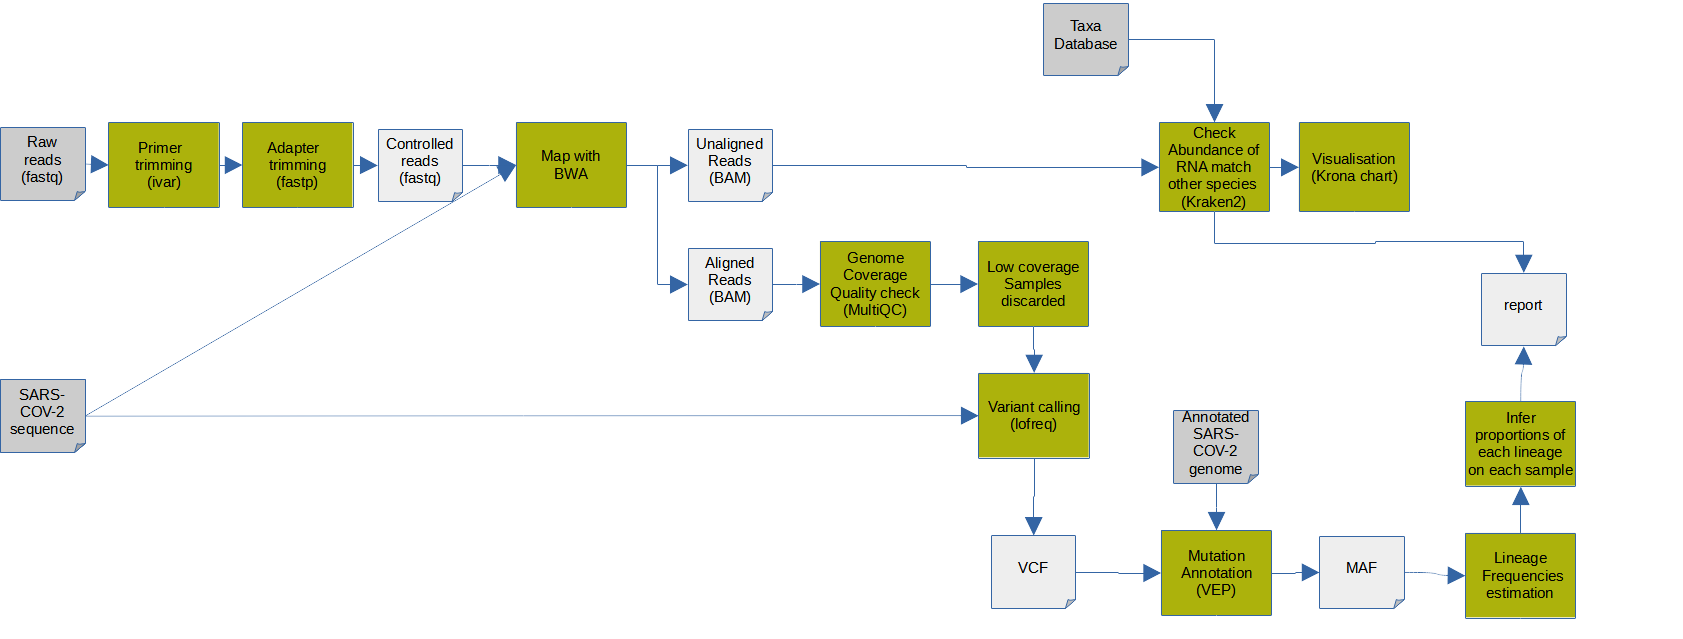
\includegraphics[width=1.5\textwidth]{figures/prior/pigx.png}
            \captionof{figure}{PiGx workflow. }
            \label{fig:prior:pigx}
        \end{figure}
        \vfill
        \end{landscape}

        \paragraph{Cowwid}
        In its turn, another approach, Cowwid \cite{jahn2021} pipeline uses steps: i) processing raw reads with the help of V-pipe \cite{posada2021} sub-workflow (performing quality controls and read filtering with FastQC and PRINSEQ \cite{babraham,prinseq}, assembly with VICUNA \cite{vicuna2012}, read alignment with BWA-MEM and ngshmmalign \cite{li2013,ngshmmalign2021} and variant calling with ShoRAH \cite{shorah}); ii) co-occurrence analysis (detecting mutation co-occurrence) with the help of COJAC \cite{jahn2022,cojac2022}; iii) building of the list of signature mutations for the variants of concern, variant mutation table, and visualization including heatmaps and curves plots generation with the help of Jupyter; iv) generation of Python script for upload to CoV-Spectrum. The diagram that describes the Cowwid workflow is presented in \cref{fig:prior:cowwid}.
        
        The advantage of Cowwid pipeline is its capability to detect lineages that are unknown as it uses COJAC tool as a co-occurance step. The other bright side of Cowwid is that its output was already experienced to be uploaded to CoV-Spectrum which means the accessibility of results and a variety of visualizations. Though, the Jupyter-based plots as well as the upload script look hard-coding, which is disadvantageous. That means that this pipeline is advanced but requires to be adjusted and generalized in order to use it for other than datasets described by K. Jahn et al. \cite{jahn2022}. 
        \begin{landscape}
        \centering\vspace*{\fill}
        \begin{figure}[ht!]
        	\centering
            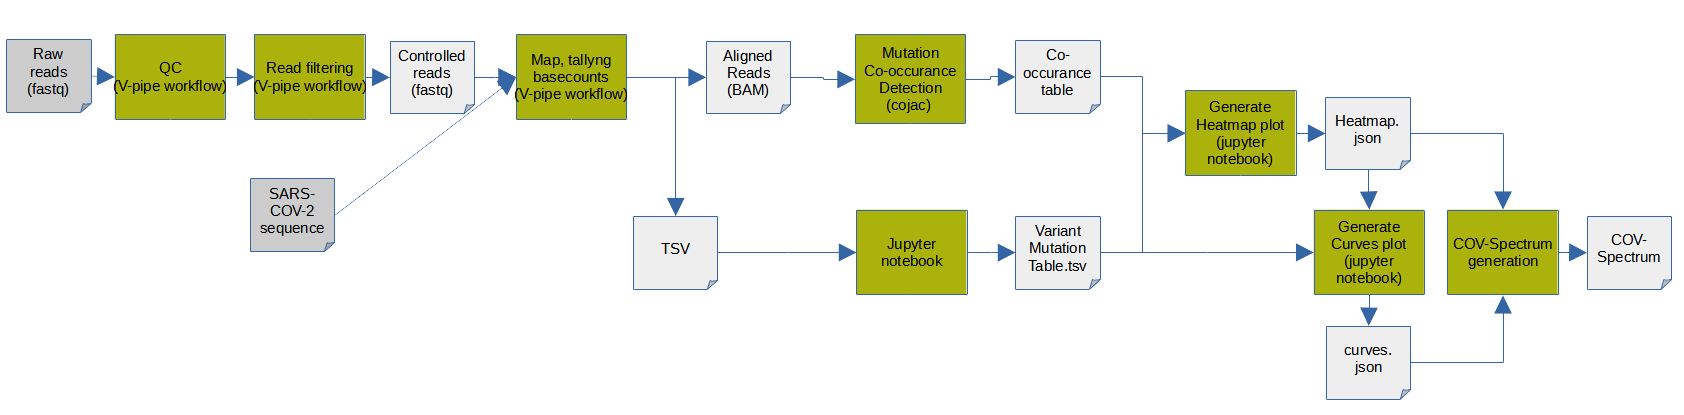
\includegraphics[width=1.4\textwidth]{figures/prior/cowwid.png}
            \captionof{figure}{Cowwid workflow.}
            \label{fig:prior:cowwid}
        \end{figure}
        \vfill
        \end{landscape}
        
        
        \paragraph{Pipeline described by R. Izquierdo-Lara et al.}
        
        Meanwhile, R. Izquierdo-Lara et al. \cite{izquierdo} used 2 different workflows using two different workflow managers (Snakemake and Galaxy). For the Nanopore data, they used Snakemake to: i) demultiplex \acrshort{fastq} raw reads using Porechop \cite{wick2022}; ii) trim of primers using Cutadapt \cite{martin2011}; iii) perform a reference-based alignment against SARS-CoV-2 reference sequence using minimap2; iv) confirm mutations in the genome by manually checking the alignment in UGENE \cite{okonechnikov2012} and resolve homopolymeric regions by consulting reference genomes. On the other hand, for the Illumina Sequence Analysis, they used Galaxy to: i) filter raw sequencing reads using Fastp \cite{chen2018}; ii) using BWA-MEM, remove adapter contamination, ambiguous bases, low quality reads (Phred score <30), and fragments <50 nt; then, map reads against GISAID sequence EPI\_ISL\_412973; iii) realign reads using FreeBayes \cite{garrison2012}; iv) generate consensus sequences and variants using iVar \cite{grubaugh2019}; v) finally, confirm variant calling by manual inspection of the aligned reads using UGENE.

        For the phylogenetic analysis, sequences were aligned with >75\% genome coverage using MAFFT \cite{mafft}, followed by visualization of trees with Figtree \cite{figtree}, and clades assignment with Nextclade tool \cite{nextclade2022}. The diagram that describes the workflow is presented in \cref{fig:prior:izquierdo}.
        
        A feature that this pipeline offers that others listed above in this section do not is phylogenetic analysis and visualization of the phylogenetic tree.
        \begin{landscape}
        \centering\vspace*{\fill}
        \begin{figure}[ht!]
        	\centering
            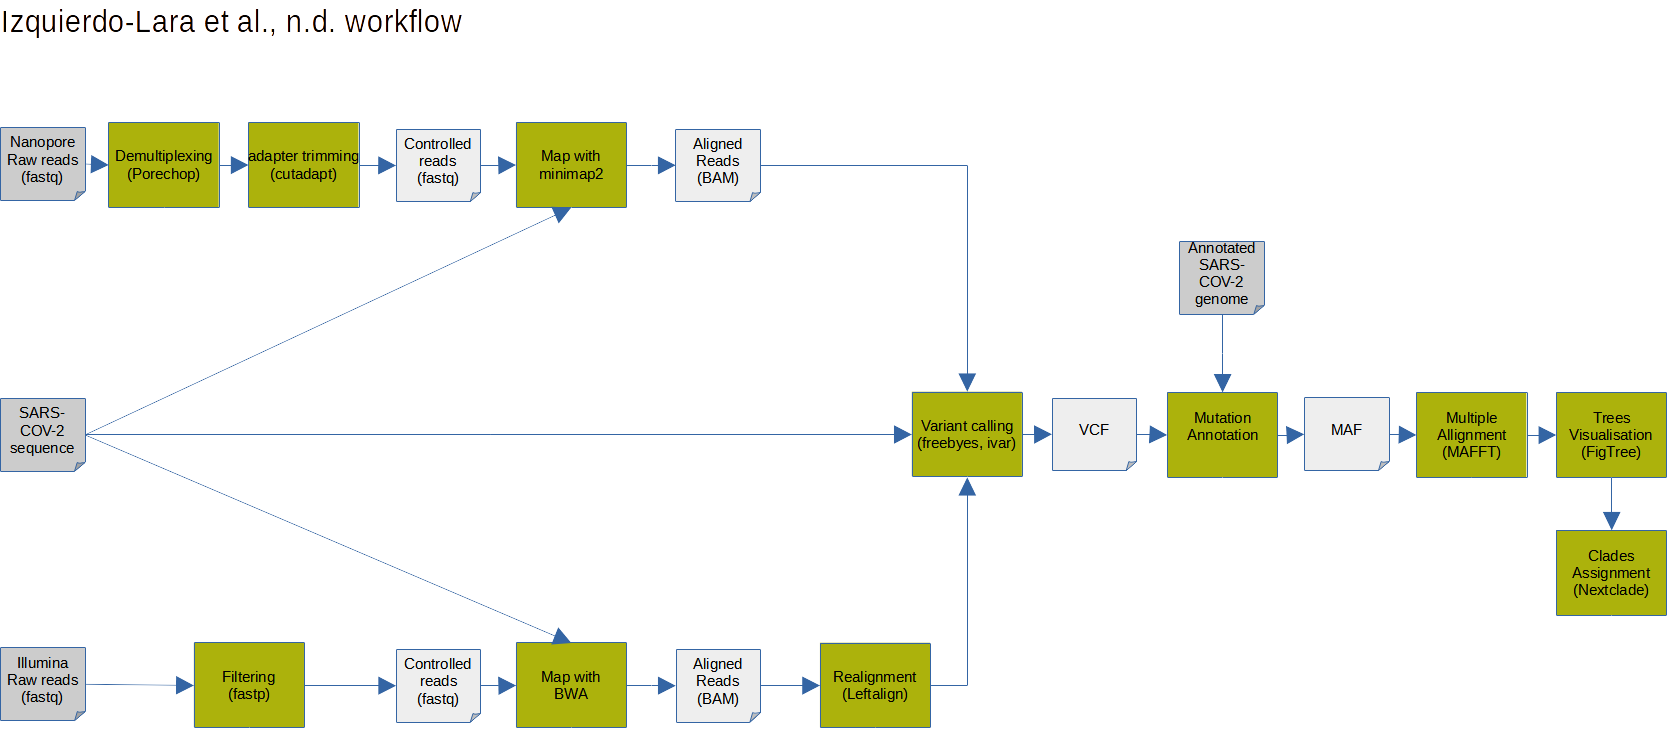
\includegraphics[width=1.4\textwidth]{figures/prior/Izquierdo-Lara.png}
            \captionof{figure}{Workflow described by R. Izquierdo-Lara et al.}
            \label{fig:prior:izquierdo}
        \end{figure}
        \vfill
        \end{landscape}
        
        
        \subsubsection{Comparison of methods for wastewater surveillance}
        To compare the existing tools and pipelines representing different state-of-the-art approaches, \cref{tab:prior:methods-tools} for individual tools and \cref{tab:prior:methods-pipelines} for standalone pipelines show some of them accompanied by source code link, license type, external tools used, description of inputs, produced outputs, their availability in Bioconda, availability in Galaxy before starting this thesis, and, finally, their prior usage (applications).
        \begin{landscape}
            \centering\vspace*{\fill}
                \begin{table}[ht!]
                \tiny
                \begin{tabular}{l|l|l|l|l|l|l|l|l|l}
\multicolumn{1}{m{1cm}|}{\textbf{Name}}&\multicolumn{1}{m{1cm}|}{\textbf{Source code}}&\multicolumn{1}{m{1cm}|}{\textbf{License}}&\multicolumn{1}{m{3cm}|}{\textbf{Goal}}&\multicolumn{1}{m{3cm}|}{\textbf{External tools plugged}}&\multicolumn{1}{m{3cm}|}{\textbf{Input}}&\multicolumn{1}{m{3cm}|}{\textbf{Output}}&\multicolumn{1}{m{1cm}|}{\textbf{Available in Bioconda}}&\multicolumn{1}{m{1cm}|}{\textbf{Available in Galaxy}}&\multicolumn{1}{m{1cm}}{\textbf{Applications}}\\ \hline 
\multicolumn{1}{m{1cm}|}{\textbf{Freyja}}&\multicolumn{1}{m{1cm}|}{\cite{joshuailevy2022}}&\multicolumn{1}{m{1cm}|}{BSD-2-Clause (open source)}&\multicolumn{1}{m{3cm}|}{Recover relative lineage abundances from mixed SARS-CoV-2 samples from a sequencing dataset (BAM aligned to the Hu-1 reference)}&\multicolumn{1}{m{3cm}|}{-}&\multicolumn{1}{m{3cm}|}{Variant call and sequencing depth information}&\multicolumn{1}{m{3cm}|}{TSV file that includes the lineages present, their corresponding abundances, and summarization by constellation}&\multicolumn{1}{m{1cm}|}{+}&\multicolumn{1}{m{1cm}|}{-}&\multicolumn{1}{m{1cm}}{\cite{karthikeyan2022,solismoreira2022,nutrition2022,karthikeyan2022b}}\\ \hline 
\multicolumn{1}{m{1cm}|}{\textbf{COJAC}}&\multicolumn{1}{m{1cm}|}{\cite{cojac2022}}&\multicolumn{1}{m{1cm}|}{GPL-3.0 (open source)}&\multicolumn{1}{m{3cm}|}{Analyzing co-occurrence of mutations on amplicons}&\multicolumn{1}{m{3cm}|}{-}&\multicolumn{1}{m{3cm}|}{BAM/CRAM/SAM and BED file describing the amplified regions}&\multicolumn{1}{m{3cm}|}{Total count of amplicons carrying the sites of interest, amplicons carrying mutations on all site of interest, amplicons where one mutation is missing, fraction (ratio of number of all amplicons carrying mutations on all sites of interest to total number of amplicons carrying cites of interest) }&\multicolumn{1}{m{1cm}|}{+}&\multicolumn{1}{m{1cm}|}{-}&\multicolumn{1}{m{1cm}}{\cite{jahn2022,jbc,karthikeyan2022b}}\\ \hline 
\multicolumn{1}{m{1cm}|}{\textbf{LCS}}&\multicolumn{1}{m{1cm}|}{\cite{valieris2022}}&\multicolumn{1}{m{1cm}|}{-}&\multicolumn{1}{m{3cm}|}{Lineage decomposition for SARS-CoV-2 pooled samples}&\multicolumn{1}{m{3cm}|}{-}&\multicolumn{1}{m{3cm}|}{Variant-groups definitions, raw-fastq files pooled samples, fasta file of the primers used}&\multicolumn{1}{m{3cm}|}{Lineage decomposition outputs for SARS-CoV-2 pooled samples, plots}&\multicolumn{1}{m{1cm}|}{-}&\multicolumn{1}{m{1cm}|}{-}&\multicolumn{1}{m{1cm}}{\cite{valieris2022,karthikeyan2022b}}\\ \hline 
\multicolumn{1}{m{1cm}|}{\textbf{Kallisto}}&\multicolumn{1}{m{1cm}|}{\cite{bray2016}}&\multicolumn{1}{m{1cm}|}{ BSD-2-Clause (open source)}&\multicolumn{1}{m{3cm}|}{Quantifying abundances of transcripts from RNA-Seq data, or more generally of target sequences using high-throughput sequencing reads}&\multicolumn{1}{m{3cm}|}{-}&\multicolumn{1}{m{3cm}|}{FASTQ (single-end or paired-end reads)}&\multicolumn{1}{m{3cm}|}{Abundance estimates, bootstrap estimates, and transcript length information length}&\multicolumn{1}{m{1cm}|}{+}&\multicolumn{1}{m{1cm}|}{+}&\multicolumn{1}{m{1cm}}{\cite{baaijens2021,anton2022}}\\ \hline 
\multicolumn{1}{m{1cm}|}{\textbf{Alcov}}&\multicolumn{1}{m{1cm}|}{\cite{ellmen2021}}&\multicolumn{1}{m{1cm}|}{-}&\multicolumn{1}{m{3cm}|}{Abundance learning for SARS-CoV-2 variants.}&\multicolumn{1}{m{3cm}|}{-}&\multicolumn{1}{m{3cm}|}{BAM file of reads aligned to the SARS-CoV-2 reference genome}&\multicolumn{1}{m{3cm}|}{Number of reads with and without each mutation in each sample, heatmap showing the frequencies for all samples, mutations, read depth for each amplicon, plots of amplicon GC content against amplicon depth}&\multicolumn{1}{m{1cm}|}{-}&\multicolumn{1}{m{1cm}|}{-}&\multicolumn{1}{m{1cm}}{\cite{ellmen2021}}\\ \hline 
\multicolumn{1}{m{1cm}|}{\textbf{SAM refiner}}&\multicolumn{1}{m{1cm}|}{\cite{gregory2021}}&\multicolumn{1}{m{1cm}|}{GPL-3.0 (open source)}&\multicolumn{1}{m{3cm}|}{Gathering variant information from a SAM formatted files}&\multicolumn{1}{m{3cm}|}{-}&\multicolumn{1}{m{3cm}|}{SAM formatted files generated from sequencing mapping programs such as Bowtie2 or MiniMap2, FASTA formatted file for a reference sequence}&\multicolumn{1}{m{3cm}|}{Unique sequences, statistics about removed chimera, covariant deconvolution output}&\multicolumn{1}{m{1cm}|}{+}&\multicolumn{1}{m{1cm}|}{-}&\multicolumn{1}{m{1cm}}{\cite{gregory2021,gregory2022,yaglom2022}}\\ \hline 
\end{tabular}
                \caption{Comparison table of existing individual tools for wastewater surveillance} \label{tab:prior:methods-tools}
                \end{table}

\begin{table}[ht!]
                \tiny
                \begin{tabular}{l|l|l|l|l|l|l|l|l|l}
\multicolumn{1}{m{1cm}|}{\textbf{Name}}&\multicolumn{1}{m{1cm}|}{\textbf{Source code}}&\multicolumn{1}{m{1cm}|}{\textbf{License}}&\multicolumn{1}{m{3cm}|}{\textbf{Goal}}&\multicolumn{1}{m{3cm}|}{\textbf{External tools plugged}}&\multicolumn{1}{m{3cm}|}{\textbf{Input}}&\multicolumn{1}{m{3cm}|}{\textbf{Output}}&\multicolumn{1}{m{1cm}|}{\textbf{Available in Bioconda}}&\multicolumn{1}{m{1cm}|}{\textbf{Available in Galaxy}}&\multicolumn{1}{m{1cm}}{\textbf{Applications}}\\ \hline 
\multicolumn{1}{m{1cm}|}{\textbf{Pipes et al.}}&\multicolumn{1}{m{1cm}|}{\cite{pipes2022}}&\multicolumn{1}{m{1cm}|}{GPL-3.0 (open source)}&\multicolumn{1}{m{3cm}|}{Estimating the relative proportions of SARS-CoV-2 strains from wastewater samples}&\multicolumn{1}{m{3cm}|}{Bowtie2}&\multicolumn{1}{m{3cm}|}{FASTA file; MSA FASTA of SARS-CoV-2 reference strains}&\multicolumn{1}{m{3cm}|}{Estimated proportion of candidate strains, barplot with only those strains with an estimated proportion larger than 1\%}&\multicolumn{1}{m{1cm}|}{-}&\multicolumn{1}{m{1cm}|}{-}&\multicolumn{1}{m{1cm}}{\cite{pipes2022}}\\ \hline 
\multicolumn{1}{m{1cm}|}{\textbf{Grom- stole}}&\multicolumn{1}{m{1cm}|}{\cite{gromstole2022}}&\multicolumn{1}{m{1cm}|}{MIT (open source)}&\multicolumn{1}{m{3cm}|}{To estimate the relative frequencies of different SARS-CoV-2 lineages}&\multicolumn{1}{m{3cm}|}{Minimap2, Cutapapt}&\multicolumn{1}{m{3cm}|}{Paired-end reads in separate FASTQ/FASTA files, NC043312.fa as a reference genome}&\multicolumn{1}{m{3cm}|}{Counts of each mutation of the lineages, coverage at every position on the reference genome, estimate of the proportion (including 95\% confidence interval); }&\multicolumn{1}{m{1cm}|}{-}&\multicolumn{1}{m{1cm}|}{-}&\multicolumn{1}{m{1cm}}{\cite{gromstole2022}}\\ \hline 
\multicolumn{1}{m{1cm}|}{\textbf{AG}}&\multicolumn{1}{m{1cm}|}{\cite{nguessan2022}}&\multicolumn{1}{m{1cm}|}{GPL-3.0 (open source)}&\multicolumn{1}{m{3cm}|}{Analyzing the within-sample genetic diversity of SARS-CoV-2 in Wastewater samples.}&\multicolumn{1}{m{3cm}|}{Trim Galore, minimap2, SAMtools, iVar, BEDTools, Picard, FreeBayes, SnpEff}&\multicolumn{1}{m{3cm}|}{Paired-end .fastq files for each sample}&\multicolumn{1}{m{3cm}|}{Tabular files with scanned variants, common depth report}&\multicolumn{1}{m{1cm}|}{-}&\multicolumn{1}{m{1cm}|}{-}&\multicolumn{1}{m{1cm}}{\cite{nguessan2022}}\\ \hline 
\multicolumn{1}{m{1cm}|}{\textbf{Lineage- spot}}&\multicolumn{1}{m{1cm}|}{\cite{pechlivanis2022}}&\multicolumn{1}{m{1cm}|}{MIT (open source)}&\multicolumn{1}{m{3cm}|}{Identify SARS-CoV-2 related mutations based on a single (or a list) of variant(s) file(s) (i.e., variant calling format).}&\multicolumn{1}{m{3cm}|}{Trim Galore, FastQC, minimap2, SAMtools, BEDTools, Picard, FreeBayes, SnpEff}&\multicolumn{1}{m{3cm}|}{Raw fastq FASTQ files, anf for further analysis - VCF and file containing all lineage-assignment rules, as retrieved from the pangolin tool repository}&\multicolumn{1}{m{3cm}|}{VCF, MAF files, eport about lineage abundances}&\multicolumn{1}{m{1cm}|}{-}&\multicolumn{1}{m{1cm}|}{-}&\multicolumn{1}{m{1cm}}{\cite{pechlivanis2022}}\\ \hline 
\multicolumn{1}{m{1cm}|}{\textbf{PiGx}}&\multicolumn{1}{m{1cm}|}{\cite{schumann2021}}&\multicolumn{1}{m{1cm}|}{GPL-3.0 (open source)}&\multicolumn{1}{m{3cm}|}{Analyzing data from sequenced wastewater samples and identifying given lineages of SARS-CoV-2}&\multicolumn{1}{m{3cm}|}{iVAR, fastp, BWA, MultiQC, LoFreq, VEP , Kraken2, Krona}&\multicolumn{1}{m{3cm}|}{Raw reads and the additional information about used primers and adapters}&\multicolumn{1}{m{3cm}|}{VCF, visualization of the development of virus over time, variants report, taxonomic classification}&\multicolumn{1}{m{1cm}|}{-}&\multicolumn{1}{m{1cm}|}{-}&\multicolumn{1}{m{1cm}}{\cite{schumann2021}}\\ \hline 
\multicolumn{1}{m{1cm}|}{\textbf{Cowwid}}&\multicolumn{1}{m{1cm}|}{\cite{jahn2021}}&\multicolumn{1}{m{1cm}|}{-}&\multicolumn{1}{m{3cm}|}{Surveillance of SARS-CoV-2 genomic variants in wastewater}&\multicolumn{1}{m{3cm}|}{V-pipe, FastQC, PRINSEQ, VICUNA, BWA-MEM, ShoRAH, COJAC}&\multicolumn{1}{m{3cm}|}{TSV table of the samples, YAML with definition of the variants, BED with amplicon positions for ARTIC, BED with amplicon description}&\multicolumn{1}{m{3cm}|}{YAML/CSV files with coocurrences, variant mutations table, plts to integrate to CoV-Spectrum}&\multicolumn{1}{m{1cm}|}{-}&\multicolumn{1}{m{1cm}|}{-}&\multicolumn{1}{m{1cm}}{\cite{jahn2021,swisscovspectrum}}\\ \hline 
\multicolumn{1}{m{1cm}|}{\textbf{Izquierdo -Lara et al.}}&\multicolumn{1}{m{1cm}|}{\cite{izquierdo}}&\multicolumn{1}{m{1cm}|}{-}&\multicolumn{1}{m{3cm}|}{Monitoring SARS-CoV-2 Circulation and Diversity through Community Wastewater Sequencing, the Netherlands and Belgium}&\multicolumn{1}{m{3cm}|}{Porechop, Cutadapt, UGENE, Fastp, BWA-MEM, FreeBayes, iVar}&\multicolumn{1}{m{3cm}|}{Raw reads and the additional information about used primers and adapters}&\multicolumn{1}{m{3cm}|}{VCF, MAF files, Trees visualization (Fig tree)}&\multicolumn{1}{m{1cm}|}{-}&\multicolumn{1}{m{1cm}|}{-}&\multicolumn{1}{m{1cm}}{\cite{izquierdo}}\\ \hline 
                \end{tabular}
                \caption{Comparison table of existing standalone pipelines for wastewater surveillance} \label{tab:prior:methods-pipelines}
                \end{table}
                \vfill
            \end{landscape}
        

    \subsection{Discussion of existing methods} \label{sec:prior:discussion}
    A number of methods were described above that use different models to determine SARS-CoV-2 lineages and their abundances in wastewater samples. Several of the methods listed can be applied to the purpose of this thesis, i.e., improvement of existing Galaxy workflows for analyzing SARS-CoV-2 clinical samples, repurposing them to detection of SARS-CoV-2 variants in wastewater samples as well as discerning of lineage abundances in these samples. It should be pointed out that, in \cref{sec:prior:methods:tools}, separate tools are listed that focus directly on lineage abundance computation, whereas, in \cref{sec:prior:methods:pipelines}, complete and almost complete standalone pipelines like PiGx, Lineagespot, Cowwid, etc. are listed that include the entire raw reads bioinformatics analysis. Standalone pipelines are not intended to be improved in this work. Conversely, individual tools that are capable of being plugged into existing Galaxy workflows and performing lineage abundances computation are the interest of this thesis.

    Two tools, Freyja \cite{joshuailevy2022,karthikeyan2022} and COJAC \cite{jahn2021}, were a choice to use in the workflows to achieve the goal of this thesis. Roughly speaking, these tools are different in purpose; for example, Freyja’s output is easy to interpret without some specific knowledge, while COJAC requires more knowledge to be used. First of all, it demands some knowledge in programming as the output of COJAC is quite raw so far and has to be processed for downstream analysis like plotting and integrating to remote platforms such as CoV-Spectrum. Second of all, the usage of COJAC requires some knowledge of virology. Despite this, COJAC provides more detailed information and is able to detect unknown variants. These two different tools, Freyja and COJAC, target different user groups (e.g., politicians and researchers), which is interesting for this thesis's research purposes.
    
    A large part of the decision on tools was based on their ability to be integrated into existing Galaxy pipelines that use Galaxy workflow manager, which meets all crucial characteristics like transparency, accessibility, and reproducibility. Furthermore, Galaxy pipelines perform decent data preprocessing steps and have shown promising results on clinical data, making them worthy of being repurposed for wastewater data using tools such as Freyja and COJAC.